\begin{framed}

Objetivos:
\begin{itemize}
    \item Repasar la descripción de fluidos mediante ecuaciones diferenciales.
    \item Repasar las leyes de conservación.
\end{itemize}

Contenidos:
\begin{itemize}
    \item Introducción y generalidades.
    \item Repaso: cinemática de una partícula de fluido.
    \item Repaso: Ecuaciones diferenciales de conservación. 
    \begin{itemize}
        \item Masa: Continuidad.
        \item Momentum: Navier-Stokes.
        \item Energía.
    \end{itemize}
\end{itemize}

Bibliografía:
\begin{itemize}
    \item White, F. M. (2008) Mecánica de Fluidos. McGraw-Hill. Sexta edición. Secciones 4.1-4.4
    \item Fox, R. W., Pritchard, P. J. y McDonald, A. T. (2009) Introduction to Fluid Mechanics. John Wiley \& Sons. Secciones 5.1-5.4
\end{itemize}
\end{framed}

En esta primera clase veremos el análisis diferencial del movimiento de un fluido. 
Para esto, iniciaremos viendo como se describe el movimiento de un elemento diferencial de fluido, para luego aplicar las leyes de conservación de masa, cantidad de movimiento, y energía sobre el elemento diferencial.
 Este material fue visto en el curso Mecánica de Fluidos General, sin embargo lo repasamos para estar en la misma página con respecto a lo que viene hacia adelante.

\section*{Elemento diferencial en movimiento}
Digamos que tenemos un flujo y que somos capaces de hacer un pequeño cuadrado con tinta al tiempo $t=0$.
Este pequeño cuadrado servirá como nuestro elemento diferencial a analizar.
Digamos que esperamos una pequeña cantidad de tiempo $\delta t$ y le sacamos una foto \mbox{?`}Qué ocurrió con el cuadrado que dibujamos? Algo como lo que muestra la Figura \ref{fig:elemento_diferencial}
%
\begin{figure}[h!]
\centering
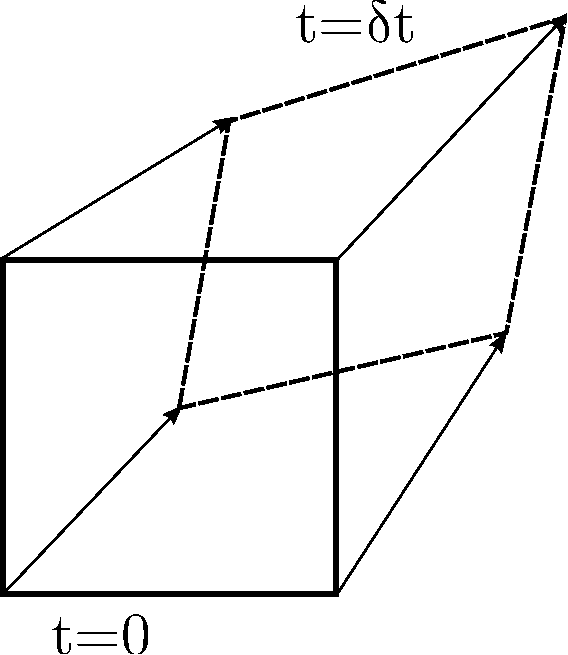
\includegraphics[width=0.4\textwidth]{clase01/elemento_diferencial.pdf}
\caption{Deformación y traslación de un elemento diferencial tras un tiempo $\delta t$}
\label{fig:elemento_diferencial}
\end{figure}

La razón por la que el elemento de fluido de la Figura \ref{fig:elemento_diferencial} se deformó es que la velocidad no es constante dentro del mismo. 
En la figura, las flechas representan el cambio de posición de las esquinas en el tiempo $\delta t$, que es el mismo en los cuatro casos, por lo que nos entregan una idea de la velocidad en esos puntos, la cual es distinta en cada caso.
De hecho, si $\delta t=1$s, las flechas serían exactamente la velocidad. 

De esta forma, podemos concluir que existe un campo de velocidad $\mathbf{V}(\mathbf{x},t) = (u(\mathbf{x},t),v(\mathbf{x},t),w(\mathbf{x},t))$, donde $\mathbf{x}=(x,y,z)$, que puede ir variando en el espacio y tiempo.

\subsubsection*{Campo de velocidades}
